\documentclass[../../main.tex]{subfiles}
\begin{document}

{\bf [解答]}

% 題意の点の配置
\begin{figure}[htb]
  \centering
  \begin{tikzpicture}[scale=3.6, >=stealth, every node/.style={font=\small}]

    % --- 1. 定数・幾何パラメータ ---
    % 中心 A(1/2, 0), 半径 1/2 の円: |z - 1/2| = 1/2
    % 円周上の点 P(alpha) と Q(beta)
    % phi_P = 65°: P ≈ (0.7113, 0.4532)
    % phi_Q = 145°: Q ≈ (0.0904, 0.2868)
    \pgfmathsetmacro{\xP}{0.5 + 0.5*cos(65)}
    \pgfmathsetmacro{\yP}{0.5*sin(65)}
    \pgfmathsetmacro{\xQ}{0.5 + 0.5*cos(145)}
    \pgfmathsetmacro{\yQ}{0.5*sin(145)}

    \coordinate (O)      at (0, 0);
    \coordinate (Center) at (0.5, 0);
    \coordinate (P)      at (\xP, \yP);
    \coordinate (Q)      at (\xQ, \yQ);

    % 直線 PQ: (yP - yQ)*x - (xP - xQ)*y + (xP*yQ - yP*xQ) = 0
    % 原点 O(0,0) から直線 PQ への垂線の足 R の座標計算
    \pgfmathsetmacro{\dx}{\xP - \xQ}
    \pgfmathsetmacro{\dy}{\yP - \yQ}
    \pgfmathsetmacro{\cross}{\xP*\yQ - \yP*\xQ}
    \pgfmathsetmacro{\denom}{\dx*\dx + \dy*\dy}
    \pgfmathsetmacro{\xR}{-\dy * \cross / \denom}
    \pgfmathsetmacro{\yR}{\dx * \cross / \denom}
    \coordinate (R) at (\xR, \yR);

    % 直線 PQ の傾き角
    \pgfmathsetmacro{\angPQ}{atan2(\dy, \dx)}

    % --- 2. 軌跡の円 |z - 1/2| = 1/2 ---
    \fill[blue!6, opacity=0.8] (Center) circle (0.5);
    \draw[thick, dashed, blue!70!black] (Center) circle (0.5);
    \node[blue!85!black, font=\scriptsize, above left] at (0.25, 0.48)
    {$\left|z - \frac{1}{2}\right| = \frac{1}{2}$};

    % --- 3. 座標軸 (複素数平面: 実軸 Re, 虚軸 Im) ---
    \draw[->, thick, gray!80!black] (-0.3, 0) -- (1.45, 0) node[right] {$\text{Re}$};
    \draw[->, thick, gray!80!black] (0, -0.25) -- (0, 1.15) node[above] {$y$ (Im)};
    \node[below left=2pt] at (O) {$O$};

    % --- 4. 直線 l (PQ を通る直線) ---
    \draw[line width=1.5pt, gray!75!black] ($ (P)!-0.45!(Q) $) -- ($ (P)!1.35!(Q) $)
    node[above right=-1pt, font=\footnotesize, black] {直線 $l$};

    % --- 5. 垂線 OR ---
    \draw[line width=1.8pt, red!85!black] (O) -- (R);
    \node[red!90!black, font=\scriptsize\bfseries, below right] at ($ (O)!0.5!(R) $) {垂線 $OR$};

    % --- 6. 直角記号 (OR ⊥ PQ) ---
    \draw[thin, red!80!black]
    ($ (R) + ({\angPQ}:0.07) $) --
    ($ (R) + ({\angPQ}:0.07) + ({\angPQ - 90}:0.07) $) --
    ($ (R) + ({\angPQ - 90}:0.07) $);

    % --- 7. 目盛りと主要点のプロット ---
    \draw[dotted, gray!60] (Center) -- (0.5, -0.08);
    \node[below=2pt, font=\scriptsize] at (Center) {$\frac{1}{2}$};
    \node[below=2pt, font=\scriptsize] at (1.0, 0) {$1$};
    \node[circle, fill, inner sep=0.6pt] at (Center) {};
    \node[circle, fill, inner sep=0.6pt] at (1.0, 0) {};

    % 点 P(alpha), Q(beta), R(w)
    \node[circle, fill, inner sep=1.2pt] at (P) {}; \node[above right=1pt] at (P) {$P(\alpha)$};
    \node[circle, fill, inner sep=1.2pt] at (Q) {}; \node[above left=1pt] at (Q) {$Q(\beta)$};
    \node[circle, fill=red!85!black, inner sep=1.4pt] at (R) {}; \node[above=2pt, red!90!black] at (R) {$R(w)$};

  \end{tikzpicture}
  \caption{直線 $PQ$ への原点からの垂線の足 $R(w)$ と円 $\left|z - \dfrac{1}{2}\right| = \dfrac{1}{2}$}
  \label{fig:complex_orthogonal_projection_safe}
\end{figure}

\begin{figure}[htb]
  \centering
  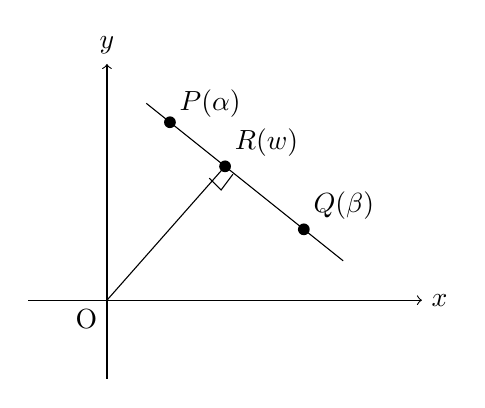
\begin{tikzpicture}
    \draw[->] (-1,0) -- (4,0) node[right] {$x$};
    \draw[->] (0,-1) -- (0,3) node[above] {$y$};
    \node at (0,0) [below left] {O};
    \draw (0.5,2.5) -- (3,0.5);
    \node at (0.8,2.2) [above right] {$P(\alpha)$};
    \node[circle, fill, inner sep=1.5pt] at (0.8,2.26) {};
    \node at (2.5,0.9) [above right] {$Q(\beta)$};
    \node[circle, fill, inner sep=1.5pt] at (2.5,0.9) {};
    \draw (0,0) -- (1.5,1.7);
    \node at (1.5,1.7) [above right] {$R(w)$};
    \node[circle, fill, inner sep=1.5pt] at (1.5,1.7) {};
    \draw (1.3,1.55) -- (1.45,1.4) -- (1.6,1.6);
  \end{tikzpicture}
  \caption{点$P(\alpha),Q(\beta),R(w)$の配置}
\end{figure}

直線$OR$が直線$PQ$の垂線だからこれら二つは直交する．従って
\begin{align}
  \dfrac{w}{\alpha - \beta} \text{ は純虚数} \label{eq:1}
\end{align}
である．

さらに点$R$は $l$ 上だから，$t \in \mathbb{R}$ として
\begin{align}
  (w - \beta) = t(\alpha - \beta) \\
  \therefore
  \dfrac{w-\beta}{\alpha-\beta} \in \mathbb{R} \label{eq:2}
\end{align}
である．\cref{eq:1,eq:2}から
\begin{align}
  &
  \begin{cases}
    \left( \dfrac{w}{\alpha-\beta} \right) + \overline{\left( \dfrac{w}{\alpha-\beta} \right)} = 0 \\
    \left( \dfrac{w-\beta}{\alpha-\beta} \right) = \overline{\left( \dfrac{w-\beta}{\alpha-\beta} \right)}
  \end{cases} \\
  \therefore
  &
  \begin{cases}
    w(\bar{\alpha}-\bar{\beta}) + \bar{w}(\alpha-\beta) = 0  \\
    (w-\beta)(\bar{\alpha}-\bar{\beta}) = (\bar{w}-\bar{\beta})(\alpha-\beta)
  \end{cases} \label{eq:3}
\end{align}
である．

まず $w \neq 0$ だから\cref{eq:3}の第一式より
\begin{align}
  \bar{\alpha}-\bar{\beta} &= -\dfrac{\bar{w}}{w}(\alpha-\beta)
\end{align}
だから\cref{eq:3}の第二式に代入して，
\begin{align}
  -(w-\beta)\dfrac{\bar{w}}{w}(\alpha-\beta) = (\bar{w}-\bar{\beta})(\alpha-\beta)
\end{align}
となる．$\alpha \neq \beta, w \neq 0$ より両辺$\alpha-\beta$で割って
\begin{align}
  & -(w-\beta)\bar{w} = w(\bar{w}-\bar{\beta}) \\
  & 2|w|^2 - \bar{\beta}w - \beta\bar{w} = 0  \label{eq:4}
\end{align}
である．

同様にして，\cref{eq:2}で
\begin{align}
  \dfrac{w-\alpha}{\beta-\alpha} \in \mathbb{R}
\end{align}
でもあるから，\cref{eq:4}までと同様の手順で
\begin{align}
  2|w|^2 - \bar{\alpha}w - \alpha\bar{w} &= 0 \label{eq:5}
\end{align}
を得る．

以下$w=\alpha\beta$となる必要十分条件を考える．

\subparagraph{$1^\circ$ 十分性}

$w = \alpha\beta$ の時，\cref{eq:4,eq:5}に代入して
\begin{align}
  \begin{cases}
    2|\alpha|^2|\beta|^2 - \alpha|\beta|^2 - \bar{\alpha}|\beta|^2 = 0 \\
    2|\alpha|^2|\beta|^2 - \beta|\alpha|^2 - \bar{\beta}|\alpha|^2 = 0
  \end{cases}
\end{align}
であり，$\alpha, \beta \neq 0$ だから，
\begin{align}
  \begin{cases}
    \left|\alpha - \dfrac{1}{2}\right|^2 = \dfrac{1}{4} \\
    \left|\beta - \dfrac{1}{2}\right|^2 = \dfrac{1}{4}
  \end{cases}
\end{align}
となり，各辺 $0$ 以上だから
\begin{align}
  \left|\alpha - \dfrac{1}{2}\right| = \dfrac{1}{2},
  \left|\beta - \dfrac{1}{2}\right| = \dfrac{1}{2}
\end{align}
より，$P(\alpha), Q(\beta)$ は題意の円周上にある．よって十分である．

\subparagraph{$2^\circ$ 必要性}

$\alpha,\beta$が中心$A(1/2)$, 半径$1/2$の円周上にあるから
\begin{align}
  \begin{cases}
    \left|\alpha - \dfrac{1}{2}\right|^2 = \dfrac{1}{4} \\
    \left|\beta - \dfrac{1}{2}\right|^2 = \dfrac{1}{4}
  \end{cases}
\end{align}
が成立する．変形すると
\begin{align}
  \begin{cases}
    \bar{\alpha} = \dfrac{\alpha}{2\alpha-1} \\
    \bar{\beta} = \dfrac{\beta}{2\beta-1}
  \end{cases} \quad \left(\because \alpha, \beta \neq \dfrac{1}{2}\right) \label{eq:6}
\end{align}
である．

$A = \alpha - \beta$ とおく．$\alpha \neq \beta$ より $A \neq 0$ だから\cref{eq:3}の第一式より
\begin{align}
  \bar{w} = -\dfrac{\bar{A}}{A}w
\end{align}
だから\cref{eq:3}の第二式に代入して
\begin{align}
  \left(-\dfrac{\bar{A}}{A}w - \bar{\beta}\right)A &= (w - \beta)\bar{A} \\
  -\bar{A}w - \bar{\beta}A &= \bar{A}w - \beta\bar{A} \\
  \beta\bar{A} - \bar{\beta}A &= 2\bar{A}w
\end{align}
を得る．$w$について整理して
\begin{align}
  w
  &= \dfrac{\beta\bar{A} - \bar{\beta}A}{2\bar{A}} \\
  &= \dfrac{\beta}{2} - \dfrac{1}{2} \left( \dfrac{\beta}{2\beta-1} \right) \dfrac{\alpha-\beta}{\dfrac{\alpha}{2\alpha-1} - \dfrac{\beta}{2\beta-1}} \quad (\because \text{\cref{eq:6}}) \\
  &= \dfrac{\beta}{2} - \dfrac{1}{2} (2\alpha-1)\beta = \alpha\beta
\end{align}
を得る．
\casesend

以上 $1^\circ$，$2^\circ$ から題意は示された．

\end{document}
